\documentclass[10pt]{beamer}
\usetheme[progressbar=frametitle]{metropolis} 
\setbeamertemplate{frame numbering}[fraction]
\setbeamertemplate{footline}{\insertshorttitle\insertshortsubtitle\hfill\insertshortauthor\hspace*{2em}\insertframenumber/\inserttotalframenumber\hspace*{2em}\vskip2pt}
% Packages
\usepackage{graphicx}
\usepackage{amsmath}
\usepackage{hyperref}
\usepackage{amsthm}
\usepackage[spanish]{babel}

\usepackage[most]{tcolorbox}

% Environments and boxes
\newtcolorbox{cajita}[1][]{
	#1
}

\newenvironment{sol}
{\renewcommand\qedsymbol{$\square$}\begin{proof}[\textbf{Solución.}]}
	{\end{proof}}

\newenvironment{dem}
{\renewcommand\qedsymbol{$\blacksquare$}\begin{proof}[\textbf{Demostración.}]}
	{\end{proof}}

\newtheorem{problema}{Problema}
\newtheorem{definicion}{Definición}
\newtheorem{ejemplo}{Ejemplo}
\newtheorem{teorema}{Teorema}
\newtheorem{corolario}{Corolario}[teorema]
\newtheorem{lema}[teorema]{Lema}
\newtheorem{prop}{Proposición}
\newtheorem*{nota}{\textbf{NOTA}}
\renewcommand\qedsymbol{$\blacksquare$}

% Set color of title, subtitle, author, institute, and date to white
\setbeamercolor{title}{fg=white}
\setbeamercolor{subtitle}{fg=white}
\setbeamercolor{author}{fg=white}
\setbeamercolor{institute}{fg=white}
\setbeamercolor{date}{fg=white}
% Title Page

\title{ Geometría diferencial}
\subtitle{ - Superficies mínimas: Helicoide y Catenoide ¿cuál es su relación?}
\author{Rudik Rompich}
\institute{Universidad del Valle de Guatemala }
\date{\today}
\begin{document}

\usebackgroundtemplate{

\includegraphics[width=\paperwidth,height=\paperheight]{imagenes/wallpaper.png}
}
\maketitle
\usebackgroundtemplate{}


\begin{frame}{Índice}
\setbeamertemplate{section in toc}[sections numbered]
\tableofcontents[hideallsubsections]
\end{frame}

\section{Introducción }


\section{Historia y parametrizaciones }

  %------------------------


    \begin{frame}
      \frametitle{1. Descubrimiento de Euler (1744)}
      El Catenoide fue descubierto por primera vez por el matemático suizo Leonhard Euler en 1744. Describió el Catenoides como una curva catenaria en rotación.
      \[x(u, v) = (a\cosh(v)\cos(u), a\cosh(v)\sin(u), av)\]
      \[ 0<u<2\pi, -\infty<v<\infty\]
    \end{frame}

      
      \begin{frame}
      \frametitle{Catenoide}
      \begin{figure}
      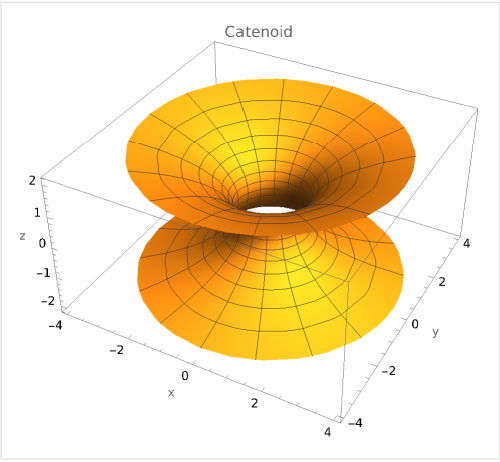
\includegraphics[scale=0.4]{imagenes/1.png}
      \caption{El Catenoide $x(u, v) = (a\cosh v \cos u, acosh v sin u, av),
      0<u<2\pi, -\infty<v<\infty$}
      \end{figure}
      \end{frame}

      \begin{frame}
        \frametitle{Catenoide}
\begin{align*}
x_u & = (-a \cosh(v) \sin(u), a \cos(u) \cosh(v), 0) \\
x_v & = (a \cos(u) \sinh(v), a \sin(u) \sinh(v), a) \\
x_{uu} & = (-a \cos(u) \cosh(v), -a \cosh(v) \sin(u), 0) \\
x_{vv} & = (a \cos(u) \cosh(v), a \cosh(v) \sin(u), 0) \\
x_{uv} = x_{vu} & = (-a \sin(u) \sinh(v), a \cos(u) \sinh(v), 0) \\
N & = \left(\frac{a^2 \cos(u) \cosh(v)}{\sqrt{a^4 \cosh^2(v)}}, \frac{a^2 \cosh(v) \sin(u)}{\sqrt{a^4 \cosh^2(v)}}, \frac{-a^2 \cosh(v) \sinh(v)}{\sqrt{a^4 \cosh^2(v)}}\right)\\
&= (\cos(u), \sin(u), -\sinh(v))
\end{align*}

        \end{frame}
        \begin{frame}
          \frametitle{Catenoide}
  \begin{align*}
  E & = a^2 \cos^2(u) \cosh^2(v) + a^2 \cosh^2(v) \sin^2(u) = a^2 \cosh^2(v) \\
  F & = 0 \\
  G & = a^2 + a^2 \cos^2(u) \sinh^2(v) + a^2 \sin^2(u) \sinh^2(v) = a^2 \cosh^2(v)\\
  e & = -\frac{a^3 \cos^2(u) \cosh^2(v) + a^3 \cosh^2(v) \sin^2(u)}{a^2 \cosh(v)}=-a \cosh(v) \\
  f & = 0 \\
  g & = \frac{a^3 \cos^2(u) \cosh^2(v) + a^3 \cosh^2(v) \sin^2(u)}{a^2 \cosh(v)} = a \cosh(v)
  \end{align*}
  
          \end{frame}

      \begin{frame}
        \frametitle{2. Observación de Meusnier (1776)}
        Jean Baptiste Meusnier demostró que el Helicoide y el Catenoide son localmente isométricos. 
        \[
        x(u, v) = (a\sinh(v)\cos(u), a\sinh(v)\sin(u), au)
        \]
        \end{frame}


      \begin{frame}
        \frametitle{Helicoide}
        \begin{figure}
        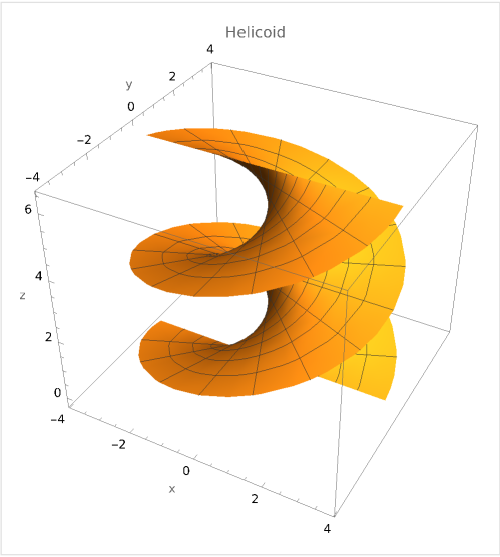
\includegraphics[scale=0.4]{imagenes/2.png}
        \caption{El Helicoide $x(u, v) = (a\sinh v\cos u, a\sinh v \sin u, au)$}
        \end{figure}
      \end{frame}

      \begin{frame}
        \frametitle{Helicoide}
        \begin{align*}
          x_u &= \left(-a \sin(u) \sinh(v), a \cos(u) \sinh(v), a\right) \\
          x_v &= \left(a \cos(u) \cosh(v), a \cosh(v) \sin(u), 0\right) \\
          x_{uu} &= \left(-a \cos(u) \sinh(v), -a \sin(u) \sinh(v), 0\right) \\
          x_{vv} &= \left(a \cos(u) \sinh(v), a \sin(u) \sinh(v), 0\right) \\
          x_{uv} &= \left(-a \cosh(v) \sin(u), a \cos(u) \cosh(v), 0\right) \\
          x_{vu} &= \left(-a \cosh(v) \sin(u), a \cos(u) \cosh(v), 0\right) \\
          N &= \left(-\frac{a\cosh(v) \sin(u)}{\sqrt{(\cosh(v)^2 + \sinh(v)^2)}}, \frac{a\cos(u) \cosh(v)}{\sqrt{(\cosh(v)^2 + \sinh(v)^2)}},\right.\\
          & \ \left. \frac{-a\cosh(v) \sinh(v)}{\sqrt{(\cosh(v)^2 + \sinh(v)^2)}}\right)
          \end{align*}
      \end{frame}

      \begin{frame}
        \frametitle{Helicoide}
        \begin{align*}
          E &= a^2 + a^2 \cos(u)^2 \sinh(v)^2 + a^2 \sin(u)^2 \sinh(v)^2= a^2\cosh (v)^2 \\
          F &= 0 \\
          G &= a^2 \cos(u)^2 \cosh(v)^2 + a^2 \sin(u)^2 \cosh(v)^2 = a^2\cosh (v)^2\\
          e &= 0 \\
          f &= \frac{a^2\cosh(v)^2}{\sqrt{(\cosh(v)^2 + \sinh(v)^2)}} \\
          g &= 0
          \end{align*}
      \end{frame}

        \begin{frame}
          \frametitle{3. Teorema de Bonnet (1848) y 4. Alternativas de Schwarz (1865)}
          Pierre Ossian Bonnet mostró que existe una familia de superficies mínimas que contiene al Catenoide y al Helicoide \footnote{Bonnet, P. O. (1867). Mémoire sur la théorie générale des surfaces. Journal de l’École Polytechnique, 32, 1-151.          }. Hermann Amandus Schwarz definió un proceso para alternar entre el Catenoides y el Helicoides, conocido como "Alternativas de Schwarz"\footnote{Schwarz, H. A. (1865). Bestimmung einer speziellen Minimalfläche. Abhandlungen der Königlichen Akademie der Wissenschaften zu Berlin, 1865, 297-326.}.
          
          \end{frame}

          \begin{frame}
            \frametitle{5. Teoría de Superficie Mínima de Hoffman y Meeks (1980s)}
            David Hoffman y William H. Meeks III hicieron contribuciones significativas a la teoría de superficies mínimas. Descubrieron nuevos ejemplos de superficies mínimas incrustadas completas y proporcionaron nuevas percepciones sobre la relación entre Catenoides y Helicoides \footnote{Hoffman, D., \& Meeks III, W. H. (1990). Embedded minimal surfaces of finite topology. Annals of Mathematics, 131(1), 1-34.}.
            \end{frame}
  %------------------------

\section{Propiedades importantes e interesantes}

\begin{frame}{Propiedades Importantes e Interesantes: Isometría Local}
  \begin{itemize}
      \item El catenoide y el helicoide son localmente isométricos.
      \item Es decir, existe una correspondencia uno a uno entre los puntos de estas dos superficies que preserva las distancias.
      \item Específicamente, las longitudes de las curvas se conservan bajo una transformación que mapea una superficie a la otra.
  \end{itemize}
  \end{frame}

\begin{frame}
  \frametitle{Proposición 1}
  \begin{cajita}
    \begin{prop}[4.2 - Do Carmo]
      Asuma la existencia de parametrizaciones $\mathbf{x}: \mathrm{U} \rightarrow \mathrm{S}$ y $\overline{\mathbf{x}}: \mathrm{U} \rightarrow \overline{\mathrm{S}}$ tal que $\mathrm{E}=\overline{\mathrm{E}}, \mathrm{F}=\overline{\mathrm{F}}, \mathrm{G}=\overline{\mathrm{G}}$ en $\mathrm{U}$. Entonces, el mapa $\varphi=$ $\overline{\mathbf{x}} \circ \mathbf{x}^{-1}: \mathbf{x}(\mathrm{U}) \rightarrow \overline{\mathrm{S}}$ es una isometría local.
    \end{prop}
  \end{cajita}


  \end{frame}
  
  \begin{frame}
  \frametitle{Isometría Local: Superficie de Revolución}
  Sea $S$ una superficie de revolución y sea
  \[
  \begin{aligned}
  \mathbf{x}(u, v)=(f(v) \cos u, f(v) \sin u, g(v)), \\
  a<v<b, \quad 0<u<2 \pi, \quad f(v)>0,
  \end{aligned}
  \]
  una parametrización de $S$. Los coeficientes de la primera forma fundamental de $S$ en la parametrización $\mathbf{x}$ son dados por
  \[
  E=(f(v))^2, \quad F=0, \quad G=\left(f^{\prime}(v)\right)^2+\left(g^{\prime}(v)\right)^2 .
  \]
  \end{frame}
  
  \begin{frame}
  \frametitle{Isometría Local: Superficie de Revolución de la Catenaria}
  La superficie de revolución de la catenaria
  \[
  x=a \cosh v, \quad z=a v, \quad-\infty<v<\infty,
  \]
  tiene la siguiente parametrización:
  \[
  \begin{aligned}
  \mathbf{x}(u, v)=(a \cosh v \cos u, & a \cosh v \sin u, a v), \\
  0 & <u<2 \pi, \quad-\infty<v<\infty,
  \end{aligned}
  \]
  con respecto a la cual los coeficientes de la primera forma fundamental son
  \[
  E=a^2 \cosh ^2 v, \quad F=0, \quad G=a^2\left(1+\sinh ^2 v\right)=a^2 \cosh ^2 v .
  \]
  \end{frame}
  
  \begin{frame}
  \frametitle{Isometría Local: Helicoide}
  Una parametrización para el helicoide es dada por
  \[
  \overline{\mathbf{x}}(\bar{u}, \bar{v})=(\bar{v} \cos \bar{u}, \bar{v} \sin \bar{u}, a \bar{u}), \quad 0<\bar{u}<2 \pi,-\infty<\bar{v}<\infty .
  \]
  Hagamos el siguiente cambio de parámetros:
  \[
  \bar{u}=u, \quad \bar{v}=a \sinh v, \quad 0<u<2 \pi,-\infty<v<\infty,
  \]
  \end{frame}
  
  \begin{frame}
  \frametitle{Isometría Local: }
  El mapa es claramente uno-a-uno, y la matriz Jacobiana del cambio de variables es dada por:

\[
\begin{bmatrix}
\frac{\partial \bar{u}}{\partial u} & \frac{\partial \bar{u}}{\partial v} \\
\frac{\partial \bar{v}}{\partial u} & \frac{\partial \bar{v}}{\partial v}
\end{bmatrix}\implies 
\begin{bmatrix}
\frac{\partial u}{\partial u} & \frac{\partial u}{\partial v} \\
\frac{\partial (a \sinh v)}{\partial u} & \frac{\partial (a \sinh v)}{\partial v}
\end{bmatrix}
\]

Al calcular las derivadas parciales, obtenemos:

\[
\begin{bmatrix}
1 & 0 \\
0 & a \cosh v
\end{bmatrix}
\]

Entonces: 
  \[
  \frac{\partial(\bar{u}, \bar{v})}{\partial(u, v)}=a \cosh v
  \]
  no es cero en ninguna parte. 
  \end{frame}


  \begin{frame}
    \frametitle{Isometría Local: }
    Así, una nueva parametrización del helicoide es
    \[
    \overline{\mathbf{x}}(u, v)=(a \sinh v \cos u, a \sinh v \sin u, a u),
    \]
    con respecto a la cual los coeficientes de la primera forma fundamental son dados por
    \[
    E=a^2 \cosh ^2 v, \quad F=0, \quad G=a^2 \cosh ^2 v .
    \]
    \end{frame}
  \begin{frame}{Transformación de Meusnier: De Catenoides a Helicoides}
    \begin{itemize}
        \item La transformación permite deformar un catenoide en un helicoide y viceversa, sin necesidad de estiramiento.
        \item Parametrización de la deformación:
    \begin{align*}
    x(u,v)&=\cos \theta \,\sinh v\,\sin u+\sin \theta \,\cosh v\,\cos u\\
    y(u,v)&=-\cos \theta \,\sinh v\,\cos u+\sin \theta \,\cosh v\,\sin u\\
    z(u,v)&=u\cos \theta +v\sin \theta
    \end{align*}
        \item Donde $\theta =\pi$ corresponde a un helicoide dextrógiro, $\theta =\pm \pi /2$ corresponde a un catenoide, y $\theta =0$ corresponde a un helicoide levógiro.
    \end{itemize}
    \end{frame}
    \begin{frame}
      \frametitle{Transformación de Meusnier}
      \begin{figure}
      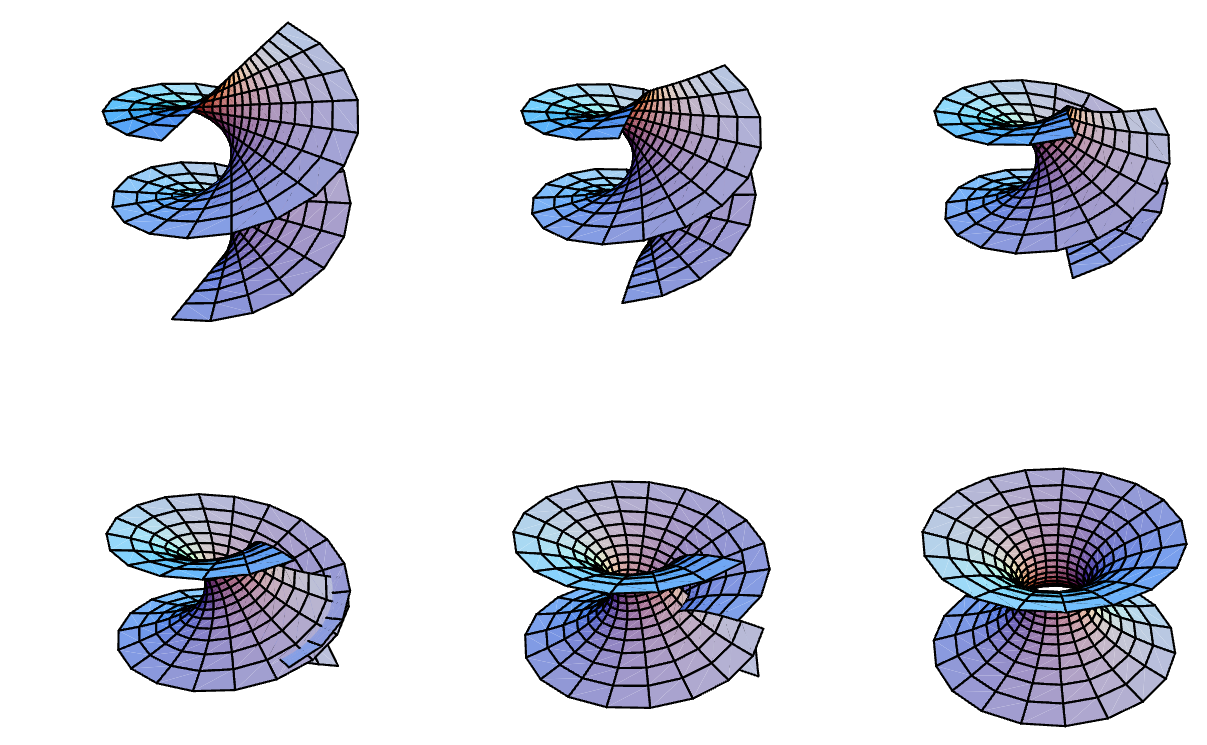
\includegraphics[scale=0.2]{imagenes/3}
      \caption{Helicoide dextrógiro, catenoide y helicoide levógiro}
      \end{figure}
      \end{frame}

  
 \section{Superficies mínimas}


 \begin{frame}
  \frametitle{Laplaciano}
  \begin{cajita}
    \begin{definicion}
      El Laplaciano \(\Delta f\) de una función diferenciable \(f: U \subset R^2 \rightarrow R\) se define por \(\Delta f=\left(\partial^2 f / \partial u^2\right)+\left(\partial^2 f / \partial v^2\right),(u, v) \in U\). Decimos que \(f\) es armónica en \(U\) si \(\Delta f=0\).
    \end{definicion}
  \end{cajita}

  \end{frame}

  \begin{frame}
    \frametitle{Superficie mínima}

    \begin{cajita}
      \begin{corolario}
        Sea \(\mathbf{x}(\mathrm{u}, \mathrm{v})=(\mathrm{x}(\mathrm{u}, \mathrm{v}), \mathrm{y}(\mathrm{u}, \mathrm{v}), \mathrm{z}(\mathrm{u}, \mathrm{v}))\) una superficie parametrizada y supongamos que \(\mathbf{x}\) es isotérmica. Entonces \(\mathbf{x}\) es mínima si y solo si sus funciones de coordenadas \(\mathrm{x}, \mathrm{y}, \mathrm{z}\) son armónicas.
      \end{corolario}
    \end{cajita}
    \end{frame}
    
  
  \begin{frame}
    \frametitle{Superficie mínima: Catenoide}

      El catenoide, dado por
  $$
  \begin{aligned}
  \mathbf{x}(u, v)=(a \cosh v \cos u, & a \cosh v \sin u, a v), \\
  & 0<u<2 \pi, \quad-\infty<v<\infty .
  \end{aligned}
  $$
  Por los problemas anteriores \(E=G=a^2 \cosh ^2 v, F=0\) y que \(\mathbf{x}_{u u}+\mathbf{x}_{v v}=0\). Por lo tanto, el catenoide es una superficie mínima.
  \end{frame}
  
  \begin{frame}
    \frametitle{Superficie mínima: Catenoide}

    Puede caracterizarse como la única superficie de revolución que es mínima.
  \end{frame}
  
  %--------------------------------

  \begin{frame}
    \frametitle{Superficie mínima: Helicoide}
    El helicoide dado por: 
    $$
    \mathbf{x}(u, v)=(a \sinh v \cos u, a \sinh v \sin u, a u) .
    $$
    Puede caracterizarse como la única superficie de revolución que es mínima. Tenemos  \(E=G=a^2 \cosh ^2 v,F=0\), y \(\mathbf{x}_{u u}+\mathbf{x}_{v v}=0\). Así, el helicoide es una superficie mínima.
  \end{frame}
  
  \begin{frame}
    \frametitle{Superficie mínima: Helicoide}

    Tiene la propiedad adicional de que
  es la única superficie mínima, aparte del plano, que también es una superficie reglada.
  \end{frame}
  

  %-------------------------------
  
  \begin{frame}{Curvatura Media Cero}
    \begin{cajita}
      \begin{definicion}
        Sea $S \subseteq \mathbb{R}^3$ superficie regular, $\mathbf{p} \in S$. Sean $\kappa_1 y \kappa_2$ las curvaturas principales de $S$ en $\mathbf{p}$. Definimos la curvatura media de $S$ en $\mathbf{p}$ como
  $$
  H=\frac{1}{2}\left(\kappa_1+\kappa_2\right)=-\frac{1}{2} \operatorname{tr} D N(\mathbf{p}) .
  $$
  Definimos la curvatura de Gauss de $S$ en $\mathbf{p}$ como
  $$
  K=\kappa_1 \kappa_2=\operatorname{det} D N(\mathbf{p})
  $$
      \end{definicion}
    \end{cajita}
    
    
 \end{frame}

 \begin{frame}{Curvatura Media Cero}

  \begin{itemize}
    \item Para una superficie mínima, la curvatura media es cero en cada punto, es decir, $H = \frac{k_1 + k_2}{2} = 0$.
    \item Por lo tanto, para el catenoide y el helicoide, las curvaturas principales en cada punto deben ser opuestas entre sí, es decir, $k_1 = -k_2$.
\end{itemize}
\end{frame}

\section{Conclusiones }


 \begin{frame}{Referencias}
  \begin{itemize}
    \item Do Carmo, M. P. (2016). Differential geometry of curves and surfaces: Revised and updated second edition. Dover Publications.
    \item Bonnet, P. O. (1867). Mémoire sur la théorie générale des surfaces. Journal de l’École Polytechnique, 32, 1-151.
    \item Schwarz, H. A. (1865). Bestimmung einer speziellen Minimalfläche. Abhandlungen der Königlichen Akademie der Wissenschaften zu Berlin, 1865, 297-326.
    \item Hoffman, D., \& Meeks III, W. H. (1990). Embedded minimal surfaces of finite topology. Annals of Mathematics, 131(1), 1-34.
  \end{itemize}
 \end{frame}



\end{document}
